We report results for all models on both the original and deduplicated datasets. Our findings show performance differences depending on tokenization, pre-training, and architecture.

\paragraph{(RQ4):} What are the contributions of the components of our \textbf{VulRepair}?

To answer this research question, we conducted an ablation study to evaluate the contribution of each component in our \textbf{VulRepair} system (Pre-training + BPE + T5), using models trained exclusively on the deduplicated dataset. We compared VulRepair against a baseline T5 model (No Pre-training + Word-level + T5), systematically varying the components to isolate their individual impact.

Specifically, we evaluated four model variants based on two factors—pre-training and tokenizer type—resulting in the following configurations:

\begin{itemize}
    \item \textbf{Pre-training + BPE + T5 (VulRepair)}: A pre-trained T5 model using Byte-Pair Encoding (BPE).
    \item \textbf{Pre-training + Word-level + T5}: A pre-trained T5 model with a word-level tokenizer.
    \item \textbf{No Pre-training + BPE + T5}: A T5 model without pre-training but using BPE.
    \item \textbf{No Pre-training + Word-level + T5}: A T5 model without pre-training and using a word-level tokenizer.
\end{itemize}

\begin{figure}[H]
    \centering
    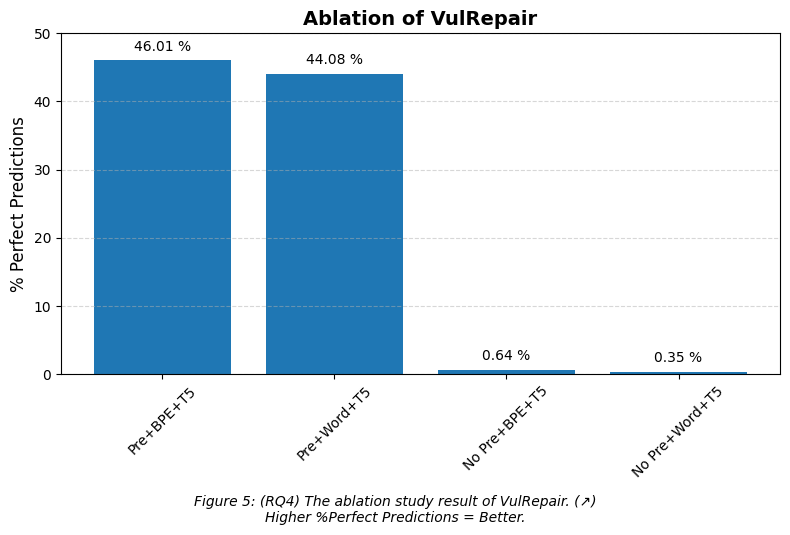
\includegraphics[width=\linewidth]{figures/rq4ablations.png}
    \label{fig:vulrepair_ablation}
\end{figure}


All variants were evaluated using the same metric: \textbf{\% Perfect Predictions}.

Result.
Figure 5 presents the ablation study conducted on the deduplicated dataset to evaluate the contributions of each component in our \textbf{VulRepair}. The results indicate that the pre-training component is the most impactful. When comparing the models with and without pre-training while keeping the BPE tokenizer fixed (Pre+BPE+T5 vs. No Pre+BPE+T5), the \%Perfect Predictions dropped from 46.01\% to 0.64\%, revealing a performance loss of approximately 45.37 percentage points.

The tokenization strategy also contributes meaningfully to the model’s effectiveness. Changing the tokenizer from BPE to word-level while keeping pre-training enabled (Pre+BPE+T5 vs. Pre+Word+T5) led to a slight reduction from 46.01\% to 44.08\%, a drop of 1.93 percentage points.

Most notably, in the absence of both pre-training and BPE tokenization (No Pre+Word+T5), the performance plummets to just 0.35\%, emphasizing the necessity of both components. These findings highlight that designing a robust Transformer-based automated vulnerability repair system like VulRepair demands not only architectural depth, but also careful attention to pre-training and tokenization strategies in order to achieve high prediction accuracy.